% Created 2024-11-07 jue 19:42
% Intended LaTeX compiler: pdflatex
\documentclass[a4paper]{article}
\usepackage[utf8]{inputenc}
\usepackage[T1]{fontenc}
\usepackage{graphicx}
\usepackage{longtable}
\usepackage{wrapfig}
\usepackage{rotating}
\usepackage[normalem]{ulem}
\usepackage{amsmath}
\usepackage{amssymb}
\usepackage{capt-of}
\usepackage{hyperref}
\usepackage[spanish]{babel}
\usepackage[usenames,dvipsnames]{color} % Required for custom colors
\renewcommand{\ttdefault}{pcr} % MONOESPACIO CON NEGRIT
\usepackage{lastpage}
\usepackage{listings}
\usepackage{listingsutf8}
\renewcommand{\lstlistingname}{Listado}
\lstset{frame=single,inputencoding=utf8,basicstyle=\scriptsize\ttfamily,showstringspaces=false,numbers=none}
\definecolor{MyDarkGreen}{rgb}{0.0,0.4,0.0} % This is the color used for comments
\lstset{ breaklines=true, postbreak=\mbox{\textcolor{red}{$\hookrightarrow$}\space}, keywordstyle=\bfseries, keywordstyle=[1]\color{Blue}\bfseries,  keywordstyle=[2]\color{Purple}\bfseries,  keywordstyle=[3]\color{Blue}\underbar,   identifierstyle=,   commentstyle=\usefont{T1}{pcr}{m}{sl}\color{MyDarkGreen}\small,   stringstyle=\color{Purple},   showstringspaces=false,   tabsize=2,   morecomment=[l][\color{Blue}]{...} }
\lstset{literate=  {á}{{\'a}}1 {é}{{\'e}}1 {í}{{\'i}}1 {ó}{{\'o}}1 {ú}{{\'u}}1   {Á}{{\'A}}1 {É}{{\'E}}1 {Í}{{\'I}}1 {Ó}{{\'O}}1 {Ú}{{\'U}}1   {à}{{\`a}}1 {è}{{\`e}}1 {ì}{{\`i}}1 {ò}{{\`o}}1 {ù}{{\`u}}1   {À}{{\`A}}1 {È}{{\'E}}1 {Ì}{{\`I}}1 {Ò}{{\`O}}1 {Ù}{{\`U}}1   {ä}{{\"a}}1 {ë}{{\"e}}1 {ï}{{\"i}}1 {ö}{{\"o}}1 {ü}{{\"u}}1   {Ä}{{\"A}}1 {Ë}{{\"E}}1 {Ï}{{\"I}}1 {Ö}{{\"O}}1 {Ü}{{\"U}}1   {â}{{\^a}}1 {ê}{{\^e}}1 {î}{{\^i}}1 {ô}{{\^o}}1 {û}{{\^u}}1   {Â}{{\^A}}1 {Ê}{{\^E}}1 {Î}{{\^I}}1 {Ô}{{\^O}}1 {Û}{{\^U}}1   {œ}{{\oe}}1 {Œ}{{\OE}}1 {æ}{{\ae}}1 {Æ}{{\AE}}1 {ß}{{\ss}}1   {ű}{{\H{u}}}1 {Ű}{{\H{U}}}1 {ő}{{\H{o}}}1 {Ő}{{\H{O}}}1   {ç}{{\c c}}1 {Ç}{{\c C}}1 {ø}{{\o}}1 {å}{{\r a}}1 {Å}{{\r A}}1   {€}{{\euro}}1 {£}{{\pounds}}1 {«}{{\guillemotleft}}1   {»}{{\guillemotright}}1 {ñ}{{\~n}}1 {Ñ}{{\~N}}1 {¿}{{?`}}1 }
\usepackage{caption}
\usepackage{attachfile2}
\usepackage[margin=1.5cm,includeheadfoot,includehead,includefoot]{geometry}
\hypersetup{colorlinks,linkcolor=black}
\usepackage{fancyhdr}
\pagestyle{fancyplain}
\chead{}
\lhead{}
\rhead{}
\cfoot{}
\lfoot{\begin{footnotesize}alvaro.gonzalezsotillo@educa.madrid.org\end{footnotesize}}
\rfoot{\begin{footnotesize}\thepage / \pageref{LastPage}\end{footnotesize}}
\usepackage[skins]{tcolorbox}
\usepackage{multicol}
\usepackage{changepage} %ajdustwidth
\usepackage{fancybox}
\usepackage{attachfile2}
\lhead{Extraordinaria 2021 (es el \\lhead)}
\rhead{Administración y Gestión de Bases de Datos (es el \\rhead)}
\lhead{IAW}
\rhead{Práctica PHP (I)}
\usepackage{svg}
\usepackage{letltxmacro}
\LetLtxMacro{\originalincludegraphics}{\includegraphics}
\renewcommand{\includegraphics}[2][]{\IfFileExists{#2.pdf}{\originalincludegraphics[#1]{#2.pdf}}{\originalincludegraphics[#1]{#2}}}
\LetLtxMacro{\originalincludesvg}{\includesvg}
\renewcommand{\includesvg}[2][]{\IfFileExists{#2.pdf}{\originalincludegraphics[#1]{#2.pdf}}{\originalincludegraphics[#1]{#2.svg.pdf}}}
\usepackage{comment}
\excludecomment{NOTES}
\date{}
\title{Primera práctica PHP}
\hypersetup{
 pdfauthor={Álvaro González Sotillo},
 pdftitle={Primera práctica PHP},
 pdfkeywords={},
 pdfsubject={},
 pdfcreator={Emacs 29.4 (Org mode 9.6.15)}, 
 pdflang={Spanish}}
\begin{document}

\maketitle
\setcounter{tocdepth}{1}
\tableofcontents

\captionsetup{font=scriptsize}

\setlength{\parindent}{0em}
\setlength{\parskip}{1em}

\newtcolorbox{Aviso}[1][Aviso]{
  enhanced,
  colback=gray!5!white,
  colframe=gray!75!black,fonttitle=\bfseries,
  colbacktitle=gray!85!black,
  attach boxed title to top left={yshift=-2mm,xshift=2mm},
  title=#1
}

\newtcolorbox{cuadrito}[1][Ignorado]{
  %drop shadow southeast,
  enhanced jigsaw,
  colback=white,
}


\newcommand{\StudentData}{
  \begin{cuadrito}[1\textwidth]
    \vspace{0.3cm}
    \large{
      \textbf{Apellidos:} \hrulefill \\
      \textbf{Nombre:} \hrulefill \\
      \textbf{Fecha:} \hrulefill \hspace{1cm} \textbf{Usuario:} \hrulefill \\
    }
    \vspace{-0.2cm}
  \end{cuadrito}
}

\section*{Objetivos de la práctica:}
\label{sec:org0000000}
En esta práctica se espera que el alumno:
\begin{itemize}
\item Se familiarice con un entorno de desarrollo PHP
\item Conozca las principales estructuras de control y funciones nativas de PHP
\end{itemize}

\section{Mazmorra Mario Bross}
\label{sec:org0000003}
Haz una función de nombre \texttt{mazmorra()} en el fichero \texttt{mazmorra.php}.
\begin{itemize}
\item Recibirá un \emph{array} de \emph{arrays}. El primer array son las filas, y el segundo las celdas dentro de las filas.
\item Se garantiza que todas las filas tienen el mismo número de celdas
\item Cada celda del array contendrá un \emph{string}, indicado el \emph{tile} que debe ponerse en la mazmorra
\item La función creará una página web con las imágenes que dibujan la mazmorra. \href{tiles/tiles.zip}{Las imágenes se pueden encontrar en este fichero ZIP}
\item Se puede usar \texttt{table}, \texttt{div}, \texttt{flex}\ldots{}
\end{itemize}

\attachfile{./tiles/tiles.zip}

\begin{lstlisting}[language=php,label= ,caption={Ejemplo de uso de \texttt{mazmorra()}},captionpos=b,numbers=none]
$tiles = [
    ["E", "E", "E", "E"],
    ["E", "T", "E", "E"],
    ["ET", "TE" "E", "T"],
    ["EI", "IT", "T","I"]
];

mazmorra($tiles);
\end{lstlisting}

\begin{figure}[htbp]
\centering

\includegraphics[width=0.5\textwidth]{tiles/ejemplo-mazmorra.png}
\caption{Resultado del listado anterior}
\end{figure}

\section{Formulario}
\label{sec:org0000006}
Crea una función de nombre \texttt{formulario()}, en el fichero \texttt{formulario.php}.
\begin{itemize}
\item Recibirá un \emph{array}.
\begin{itemize}
\item Cada clave del \emph{array} será el nombre de un campo
\item Cada valor del \emph{array} será el tipo del campo (\texttt{button}, \texttt{checkbox}, \texttt{email}, \texttt{hidden}, \texttt{number}, \texttt{password}, \texttt{search}, \texttt{submit}, \texttt{tel}, \texttt{text}\ldots{})
\end{itemize}
\item Se creará un formulario HTML con las siguientes características:
\begin{itemize}
\item Método \texttt{GET}
\item Habrá un \texttt{label} por cada campo. El texto será la clave del \emph{array}.
\item Cada campo tendrá un \texttt{name}. Será la clave del \emph{array}, cambiando espacios por \emph{underscore} (\texttt{\_})
\item Las etiquetas están a la izquierda, y los campos a la derecha, alineados en vertical.
\item Se pondrá al final un botón de \emph{submit}.
\end{itemize}
\end{itemize}


\begin{lstlisting}[language=php,label= ,caption={Ejemplo de uso de \texttt{formulario()}},captionpos=b,numbers=none]
$estructura_formulario = [
    "Nombre" => "text",
    "Email" => "email",
    "Edad" => "number",
    "Acepta politica de seguridad" => "checkbox"
];

formulario( $estructura_formulario );
\end{lstlisting}

\begin{figure}[htbp]
\centering
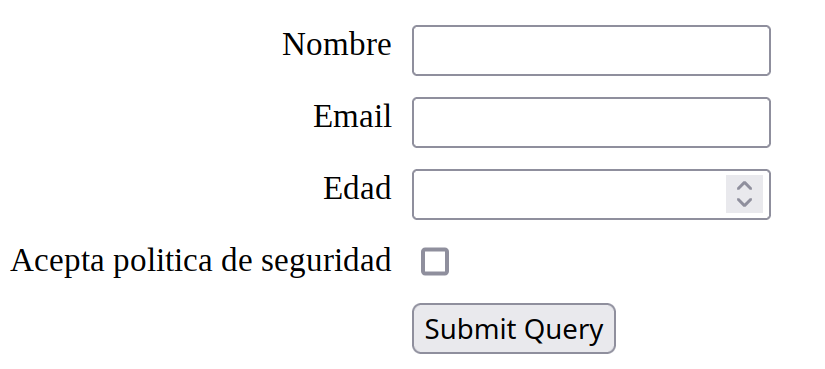
\includegraphics[width=0.5\textwidth]{tiles/ejemplo-formulario.png}
\caption{Resultado del listado anterior}
\end{figure}

\clearpage

\section{Calculadora simple}
\label{sec:org0000009}
Se creará un fichero \texttt{Calculadora.php}.
\begin{itemize}
\item Mostrará un formulario con un número con dos decimales, un selector con operaciones matemáticas, y un segundo número con dos decimales.
\begin{itemize}
\item \texttt{+}, \texttt{-}, \texttt{\%}, \texttt{/}, \texttt{*}
\end{itemize}
\item Al enviar el formulario, se mostrará el resultado de la operación. El formulario volverá a mostrar los últimos valores introducidos.
\item Si la operación no es posible, en vez del resultado se mostrará \texttt{Error}
\end{itemize}

\begin{figure}[htbp]
\centering
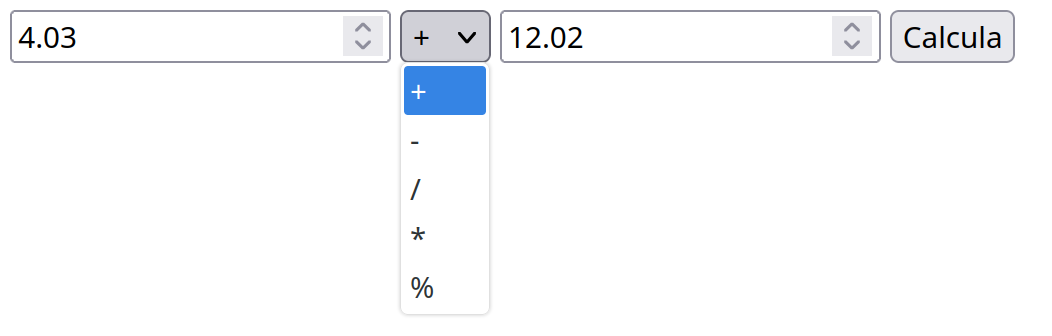
\includegraphics[width=0.5\textwidth]{tiles/ejemplo-calculadora.png}
\caption{Ejemplo de caluladora}
\end{figure}

\section*{Normas de entrega}
\label{sec:org000000c}
\begin{itemize}
\item El código estará en el directorio \texttt{\textasciitilde{}/public-html/practica01/} del \emph{workspace} de Coder del alumno
\item Los nombres de fichero PHP y los nombres de funciones serán los especificados en los enunciados
\item Se recuerda que los alumnos deben guardar una copia de seguridad de todos sus trabajos, en el caso de que Coder no funcione
\item No deben aparcer errores ni avisos de PHP. Hay que tener en cuenta que se ejecutarán con opciones de \emph{debug}, como \texttt{display\_errors} a \texttt{true}
\item Para probar los dos primeros ejercicios, el profesor incluirá un fichero como el siguiente, y lo ejecutará en en Apache del alumno
\end{itemize}


\begin{lstlisting}[language=php,label= ,caption={Ejemplo de fichero de prueba},captionpos=b,numbers=none]
<?php
ini_set('display_errors', 1);
ini_set('display_startup_errors', 1);
error_reporting(E_ALL);

include("mazmorra.php");
include("formulario.php");
?>

<div>
    <?php
    formulario(
        [
            "Nombre" => "text",
            "Email" => "email",
            "Edad" => "number",
            "Acepta politica de seguridad" => "checkbox"
        ]
    );
    ?>
 </div>

 <div>
    <?php
    mazmorra(
        [
            ["E", "E", "E", "E"],
            ["E", "T", "E", "E"],
            ["ET", "TE" "E", "T"],
            ["EI", "IT", "T","I"]
        ];
    );
    ?>
 </div>        

\end{lstlisting}

\section*{Resultados de aprendizaje}
\label{sec:org000000f}
Esta práctica contribuye a la calificación de los siguientes RA:
\begin{itemize}
\item RA 4: xx\%
\end{itemize}
\end{document}
